% oneside: Tránh tạo trang trắng thừa giữa các chương, căn lề đều nhau khi đọc PDF
\documentclass[12pt, a4paper, oneside]{book}

% --- HỖ TRỢ TIẾNG VIỆT & TOÁN HỌC ---
\usepackage[utf8]{inputenc}
\usepackage[T5]{fontenc}
\usepackage[vietnamese]{babel}
\usepackage{amsmath, amssymb}
\usepackage{graphicx}
\graphicspath{{images/}} % Tự động tìm ảnh trong thư mục images/
\usepackage{float}

% --- CĂN LỀ & KHOẢNG CÁCH ---
\usepackage[top=2.5cm, bottom=2.5cm, left=2.5cm, right=2.5cm]{geometry}
\usepackage{parskip}     % Tạo khoảng trống giữa các đoạn, không thụt đầu dòng

% --- TÙY CHỈNH MỤC LỤC (QUAN TRỌNG) ---
% tocdepth = 0: Mục lục CHỈ hiển thị cấp Chương (1 dòng cho 1 chương), ẩn hết mục con
\setcounter{tocdepth}{0} 
\usepackage[hidelinks]{hyperref} % Bấm vào tên chương ở mục lục để nhảy thẳng tới trang đó

% --- TÙY CHỈNH GẠCH ĐẦU DÒNG (-, +, •) ---
\usepackage{enumitem}
\setlist[itemize,1]{label={--}, leftmargin=1.5em}
\setlist[itemize,2]{label={+}, leftmargin=1.5em}
\setlist[itemize,3]{label={$\bullet$}, leftmargin=1.5em}

% --- THÔNG TIN CUỐN SÁCH ---
\title{\textbf{MACHINE LEARNING}}
\author{Trịnh Minh Khánh}

\begin{document}

% ================= PHẦN ĐẦU SÁCH (Đánh số trang La Mã: i, ii...) =================
\frontmatter
\maketitle          % Trang bìa
\tableofcontents    % Mục lục tự động (chỉ hiện tên chương + số trang)

% ================= PHẦN NỘI DUNG CHÍNH (Đánh số trang từ 1, 2, 3...) =================
\mainmatter
\pagestyle{plain}

% Mỗi tuần học xong, bạn chỉ cần thêm 1 dòng \input{...} vào bên dưới:
\chapter{Tổng quan về Machine Learning}

\section{Phân loại thuật toán:}
\begin{itemize}
    \item \textbf{Phương thức học}
    \item \textbf{Chức năng}
\end{itemize}


\section{Phương thức học (Learning Style)}
\begin{itemize}
    \item \textbf{Supervised Learning}
    \item \textbf{Unsupervised Learning}
    \item \textbf{Semi-Supervised Learning} 
    \item \textbf{Reinforcement Learning}
\end{itemize}
    \subsection{Supervised Learning}
    \begin{itemize}
        \item Dựa trên những dữ liệu (input, outcome) đã được học từ trước để dự đoán một dữ liệu mới (new input).
        \item Dữ liệu đã biết có dạng (data, label).
        \item Có một tập hợp biến đầu vào X và biến đầu ra Y, các cặp $(x_i, y_i)$ là các vector (tập training data). Dựa vào tập này chúng ta cần tạo hàm ánh xạ từ X sang Y có dạng $y = f(x)$ mục đích là tìm hàm xấp xỉ $f(x)$ thật tốt để phục vụ cho việc dự đoán.
        \item Bài toán được chia nhỏ thành 2 loại chính:
        \begin{itemize}
            \item Classification (Phân loại): Nếu các label của input data được chia thành một số hữu hạn nhóm.
            \item Regression (Hồi quy) : Là bài toán dự đoán một giá trị liên tục hay số thực đầu ra cho y dựa trên một hay nhiều biến đầu vào X.
        \end{itemize}
    \end{itemize}
    \subsection{Unsupervised Learning}
    \begin{itemize}
        \item Thuật toán chỉ được nhận Input
        \item Dựa vào cấu trúc dữ liệu để thực hiện một số công việc.
        \item Bài toán được chia thành 2 loại:
        \begin{itemize}
            \item Clustering (Phân nhóm):  Phân nhóm toàn bộ dữ liệu thành các nhóm nhỏ dựa trên sự liên quan giữa các dữ liệu trong mỗi nhóm. vd : đối với dữ liệu của khách hàng mua hàng thì có thể có những nhóm sau:
            \begin{itemize}
                \item Cụm chi tiêu cao.
                \item Cụm mua món ăn kèm.
                \item Cụm những người thích mua hàng sale.
            \end{itemize}
            \item Association: Bài toán tìm ra quy luật trên nhiều dữ liệu cho trước.
         \end{itemize}
    \end{itemize}
    \subsection{Semi-supervised Learning(Học bán giám sát)}
    \begin{itemize}
        \item Chỉ một phần dữ liệu được gán nhãn.
    \end{itemize}
    \subsection{Reinforcement Learning(Học củng cố)}
    \begin{itemize}
        \item Là bài toán giúp cho một hệ thống tự động xác định hành vi dựa trên hoàn cảnh để đạt lợi ích cao nhất.
        \item Bài toán huấn luyện tác nhân để tác nhân tương tác nhận phản hồi từ môi trường, định nghĩa phản hồi mà môi trường sẽ trả lại cho tác nhân.
Chủ yếu áp dụng vào : Game Theory, Thuật toán cần xác định nước đi tiếp theo để đạt điểm cao nhất
        \item Chủ yếu áp dụng vào : Game Theory, Thuật toán cần xác định nước đi tiếp theo để đạt điểm cao nhất.
        \item Ví dụ áp dụng cái này vào việc huấn luyện xe tự hành: 
        \begin{itemize}
            \item Cho vào môi trường mô phỏng và đặt thêm 1 biến, biến này có vai trò cứ làm đúng chuẩn thì sẽ được cộng vào (phần thưởng), còn nếu sai thì phải trừ.
            \item Trong lúc cộng trừ thì phụ thuộc vào hành động nó thực hiện, ví dụ như đi xe lên vỉa hè thì trừ điểm nhưng ít hơn khi xe va chạm (tông xe, tông người, …), lúc va chạm người thì phải trừ đi rất nhiều để thể hiện rõ đây là một hành vi rất nghiêm trọng,.. điều này cũng tương tự trong khi làm đúng.
        \end{itemize}
    \end{itemize}
\section{Chức năng (Function)}
\begin{itemize}
    \item Regression Algorithms:
    \begin{itemize}
        \item Linear Regression
        \item Logistic Regression
        \item Stepwise Regression
    \end{itemize}
    \item Classification Regression:
    \begin{itemize}
        \item Linear Clasifier
        \item Support Vector Machine
        \item Sparse Representation-based classification (SRC)
    \end{itemize}
    \item Clustering Algorithms:
    \begin{itemize}
        \item K-means Clustering
        \item K-meidans
        \item Expectation Maximization (EM)
    \end{itemize}
\end{itemize}



\chapter{Supervised Learning Model}
\section{Mô hình:}
\begin{figure}[H]
    \centering
    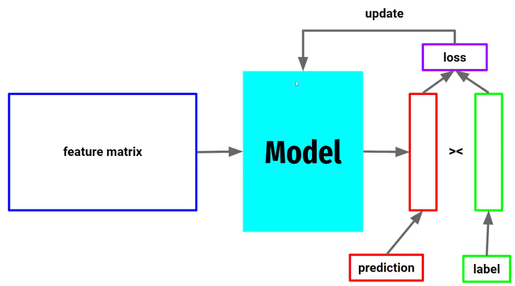
\includegraphics[width=0.8\linewidth]{01.png}
    \caption{Mô hình Supervised Learning}
    \label{fig: mdl_spl}
\end{figure}
\begin{itemize}
    \item \textbf{Giải thích mô hình:}
    \begin{itemize}
        \item Future matrix: Ma trận thuộc tính.
        \item Prediction: Kết quả từ mô hình.
        \item Label: Kết quả mong muốn.
        \item Loss: Hàm mất mát cho biết mức độ chênh lệch giữa Prediction và Label
        \begin {itemize}
            \item Loss thấp: Mô hình có độ chính xác cao.
            \item Loss cao: Ngược lại.
        \end {itemize}
        \item Loss luôn cập nhật mục đích để phản ánh lại prediction
    \end{itemize}
\end{itemize}

\section{Loss Function:}
\begin{figure}[H]
    \centering
    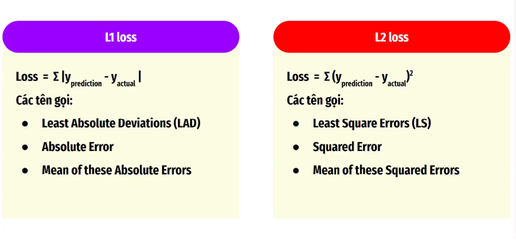
\includegraphics[width=0.8\linewidth]{02.png}
    \caption{Hàm mất mát (Loss Function)}
    \label{fig:loss_func}
\end{figure}
\subsection {Câu hỏi:}
\begin{itemize}
    \item Tại sao lại có hai hàm Loss?
    \item Sử dụng hàm như thế nào cho đúng?
\end{itemize}
\subsection {L1: Mong muốn mô hình phải thật chính xác, tối đa hoá sự chính xác:}
\begin{itemize}
    \item Thu được các sai số rất nhỏ với $y-hat$ chính xác cao.
    \item Tối đa hoá giá trị prediction với độ chính xác cao.
    \item Chấp nhận một vài outlier.
    \item Hạn chế tác động của Outlier (Không bị chi phối).
    \item Dùng cho trường hợp data bị nhiễu nhiều outlier.
\end{itemize}

\subsection {L2: Mong muốn mô hình với sai số tối thiểu, tối thiểu hoá sai số}
\begin{itemize}
    \item Sẽ nghiêm trọng với sai số lớn vì sai số sẽ bình phương lên.
    \item Mô hình sẽ tập trung vào những điểm outlier, kéo lệch kết quả dự đoán.
    \item Dùng cho bài toán có dữ liệu sạch.
\end{itemize}

\section{Phân chia dữ liệu trong ML pipeline}
\begin{figure}[H]
    \centering
    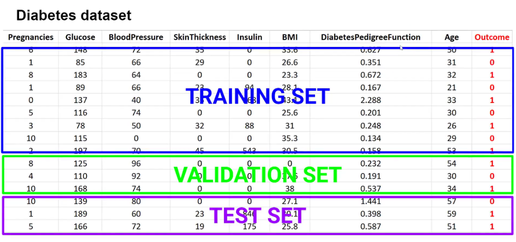
\includegraphics[width=0.8\linewidth]{03.png}
    \caption{Phân chia dữ liệu}
    \label{fig:dataset_devide}
\end{figure}

\begin{itemize}
    \item Trainning set: Dùng để huấn luyện mô hình, có khả năng làm mô hình tốt hơn nếu data càng lớn.
    \item Validation set: Kiểm tra quá trình huấn luyện, kết quả thu được dùng để cải thiện model.
    \item Test set: Kiểm tra performance của model.
\end{itemize}

\section{Classification metrics}
\begin{figure}[H]
    \centering
    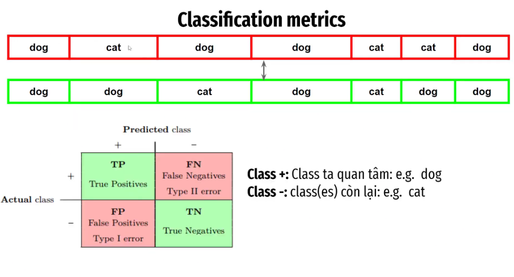
\includegraphics[width=0.8\linewidth]{04.png}
    \caption{Chia dữ liệu dựa trên mối quan tâm}
    \label{fig: class_devide}
\end{figure}
\begin{itemize}
    \item Metrics của classification: Dùng để đánh giá mô hình.
    \item Các metric thường sử dụng.
\end{itemize}
\begin{figure}[H]
    \centering
    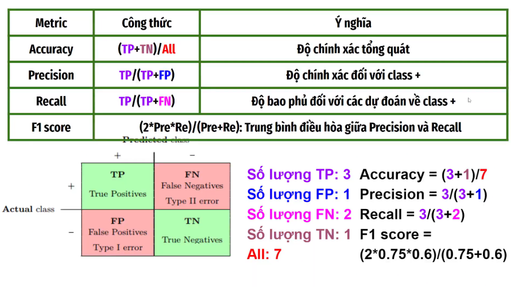
\includegraphics[width=0.8\linewidth]{05.png}
    \caption{Classification metrics}
    \label{fig:cl_metrics}
\end{figure}
\begin{itemize}
    \item Giải thích:
    \begin{itemize}
        \item Accuracy: Độ chính xác tổng quát.
        \item Precision: Đối với nhóm dương tính thì có bao nhiêu kết quả thực sự chính xác (Nhóm cụ thể).
        \item Recall: Có bao nhiêu dự đoán chính xác trên số lượng chính xác trong thực tế (Ví dụ : Trong số người thực sự dương tính  thì có bao nhiêu người được dự đoán chính xác dương tính).
        \item F1 score: Trung bình điều hòa Precision và Recall, dùng để đánh giá trong trường hợp dữ liệu mất cân bằng.
    \end{itemize}
\end{itemize}

\begin{figure}[H]
    \centering
    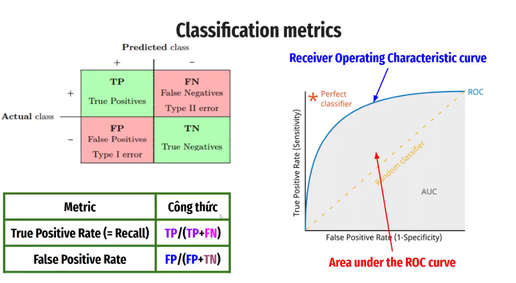
\includegraphics[width=0.8\linewidth]{06.png}
    \caption{Classification metrics}
    \label{fig:cl_metrics2}
\end{figure}
\begin{itemize}
    \item Giải thích:
    \begin{itemize}
    \item ROC: Tìm điểm tối ưu.
    \item AUC: Tìm đường tối ưu.
    \item False Positive Rate :Có bao nhiêu báo động giả(dự đoán sai) trên tổng số người âm tính thực tế. (Ví dụ : Trong tổng số người thực sự âm tính có bao nhiêu người đã bị dự đoán là dương tính).
    \end{itemize}
\end{itemize}

\begin{figure}[H]
    \centering
    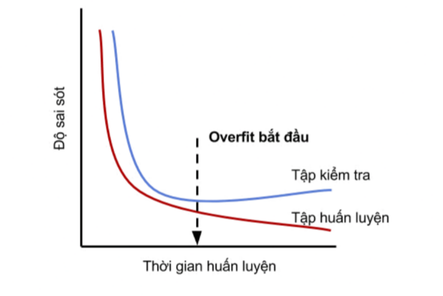
\includegraphics[width=0.8\linewidth]{07.png}
    \caption{Trainning line}
    \label{fig:trainning_line}
\end{figure}
\begin{itemize}
    \item Hiện tượng \textbf{Overfitting}: Train tốt nhưng Test kém.
    \item Ép máy tính mô phỏng lại chính xác tất cả những gì được học đồng thời cũng muốn nó có thể làm đúng được những gì chưa từng nhìn thấy dựa trên những gì đã được học, sáng tạo ra những điểm chưa tồn tại.
\end{itemize}





\chapter{Machine Learning Pipeline}

% ==========================================
% SECTION 1: ML PIPELINE
% ==========================================
\section{Quy trình Machine Learning (ML Pipeline)}

\begin{figure}[H]
    \centering
    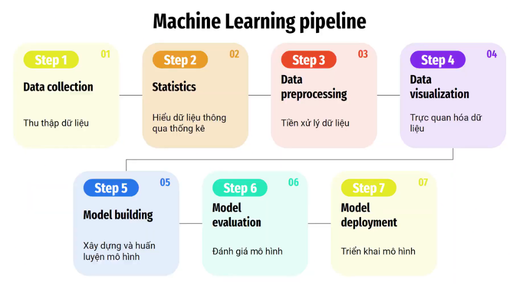
\includegraphics[width=0.8\linewidth]{11.png}
    %\fbox{\parbox[c][4cm][c]{0.8\linewidth}{\centering \textit{[Chèn ảnh: Tổng quan ML Pipeline tại đây]}}}
    \caption{Quy trình tổng quan của một ML Pipeline}
    \label{fig:ml_pipeline}
\end{figure}

\subsection{Step 1: Data Collection (Thu thập dữ liệu)}
\begin{itemize}
    \item Xác định bài toán và dữ liệu cần có.
    \item Thu thập dữ liệu.
    \item Đánh nhãn (Annotation).
    \item \textbf{OUTPUT:} Dữ liệu thô (Raw data).
\end{itemize}

\subsection{Step 2: Statistics (Thống kê mô tả)}
\begin{itemize}
    \item Thống kê: Tính toán các thông số cơ bản:
    \begin{itemize}
        \item \textbf{Mean:} Trung bình.
        \item \textbf{Median:} Trung vị.
        \item \textbf{Std:} Độ lệch chuẩn.
        \item \textbf{Variance:} Phương sai.
        \item \textbf{Min/Max:} Giá trị nhỏ nhất / lớn nhất.
        \item \textbf{Q1, Q2, Q3:} Tứ phân vị.
        \item \textbf{Mode:} Điểm dữ liệu có tần số xuất hiện lớn nhất.
    \end{itemize}
    \item \textbf{OUTPUT:} Cung cấp cái nhìn tổng quan về bộ dữ liệu.
\end{itemize}

\subsection{Step 3: Data Preprocessing (Tiền xử lý dữ liệu)}
\begin{itemize}
    \item Đưa dữ liệu về dạng máy tính có thể hiểu được (dạng số).
    \item Làm sạch dữ liệu.
    \item Chuẩn hóa: Đưa mọi tham số về cùng một thang đo.
    \item Phân chia dữ liệu: Training set, Validation set, Test set.
    \item Tạo đặc trưng mới dựa trên dữ liệu sau xử lý.
    \item Các bước trong quá trình này được xây dựng và mô hình hóa thành một pipeline/mô hình riêng, phục vụ cho các pha khác để đảm bảo tính thống nhất.
    \item \textbf{OUTPUT:} Dữ liệu đã được làm sạch, chuẩn hóa và phân chia thành từng cụm phục vụ cho từng bước.
\end{itemize}

\subsection{Step 4: Data Visualization (Trực quan hóa dữ liệu)}
\begin{itemize}
    \item Dựa trên dữ liệu cung cấp, cần trực quan hóa dữ liệu để có thể dễ dàng quan sát.
    \item Sử dụng các thư viện của python.
    \item \textbf{OUTPUT:} Biểu đồ.
\end{itemize}

\subsection{Step 5: Model Building (Xây dựng mô hình)}
\begin{itemize}
    \item Chọn thuật toán phù hợp.
    \item Tiến hành training dựa trên Training set.
    \item \textbf{Tinh chỉnh} các tham số dựa trên kết quả đầu ra.
    \item Sử dụng thêm các mô hình khác để so sánh.
    \item \textbf{OUTPUT:} Trả về mô hình đã huấn luyện, có thể dùng để dự đoán.
\end{itemize}

\subsection{Step 6: Model Evaluation (Đánh giá mô hình)}
\begin{itemize}
    \item Từ kết quả thu được trên Test set, tính toán các thông số như: Accuracy, Precision, Recall, F1 score, ROC, AUC.
    \item Kiểm tra hiện tượng Overfitting (Train tốt, Test kém).
    \item Tiến hành đánh giá kết quả của mô hình sau bài test.
    \item \textbf{OUTPUT:} Dựa vào kết quả để kết luận mô hình có đạt không. Nếu không đạt, cần xác định quay lại bước nào để tinh chỉnh.
\end{itemize}

\subsection{Step 7: Model Deployment (Triển khai mô hình)}
\begin{itemize}
    \item Tích hợp, triển khai mô hình vào các thiết bị, cloud,... để sử dụng tùy vào mục đích.
\end{itemize}

\subsection{Lưu ý về vòng lặp của Pipeline}
\begin{figure}[H]
    \centering
    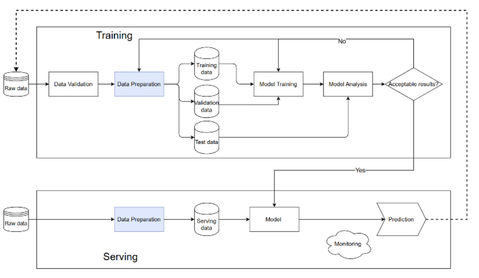
\includegraphics[width=0.8\linewidth]{12.png}
    \caption{Machine learning pipeline}
    \label{fig: hieuchinh}
\end{figure}
\begin{itemize}
    \item Pipeline thường \textbf{không chạy một chiều}, cần phải cải thiện lại nếu Step 6 chưa đạt kết quả như kỳ vọng.
    \item Đường đi phản hồi: $\text{Prediction} \rightarrow \text{Raw data}$.
    \item Nghĩa là dữ liệu thu được từ mô hình được đưa ngược về để làm Training set nhằm đảm bảo mô hình có thể bắt kịp với những thay đổi thực tế.
\end{itemize}

% ==========================================
% SECTION 2: CHI TIẾT TIỀN XỬ LÝ DỮ LIỆU
% ==========================================
\section{Các bước Tiền xử lý dữ liệu (Data Preprocessing)}

\begin{figure}[H]
    \centering
    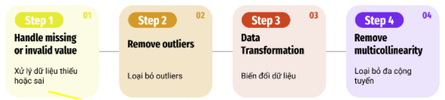
\includegraphics[width=0.8\linewidth]{13.png}
    %\fbox{\parbox[c][4cm][c]{0.8\linewidth}{\centering \textit{[Chèn ảnh: Quy trình Data Preprocessing tại đây]}}}
    \caption{Các bước chính trong tiền xử lý dữ liệu}
    \label{fig:data_preprocessing}
\end{figure}

\begin{itemize}
    \item \textbf{Step 1:} Handle missing or invalid values (Xử lý dữ liệu thiếu hoặc không hợp lệ).
    \item \textbf{Step 2:} Remove outliers (Loại bỏ các điểm ngoại lai).
    \item \textbf{Step 3:} Data transformation (Biến đổi dữ liệu):
    \begin{itemize}
        \item \textbf{Numerical feature} (Thuộc tính dạng số):
        \begin{itemize}
            \item Tiền xử lý: \texttt{MinMaxScaler} (nhạy cảm với outliers), \texttt{StandardScaler}.
            \item \textbf{Continuous:} Dữ liệu liên tục.
            \item \textbf{Discrete:} Dữ liệu rời rạc.
        \end{itemize}
        \item \textbf{Categorical feature} (Thuộc tính dạng phân loại):
        \begin{itemize}
            \item \textbf{Ordinal} (Thứ bậc) $\rightarrow$ \texttt{OrdinalEncoder}.
            \item \textbf{Nominal} (Danh nghĩa) $\rightarrow$ One-hot encoding, Hash encoding, Word Embedding.
        \end{itemize}
    \end{itemize}
    \begin{figure}[H]
    \centering
    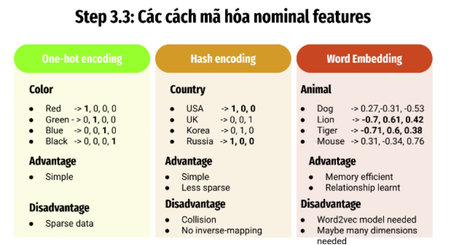
\includegraphics[width=0.8\linewidth]{14.png}
    %\fbox{\parbox[c][4cm][c]{0.8\linewidth}{\centering \textit{[Chèn ảnh: Minh họa Correlation / Multicollinearity tại đây]}}}
    \caption{Các cách mã hóa}
    \label{fig:encoder}
\end{figure}
    \item \textbf{Step 4:} Remove multicollinearity (Loại bỏ hiện tượng đa cộng tuyến).
\end{itemize}

% ==========================================
% SECTION 3: TƯƠNG QUAN & ĐA CỘNG TUYẾN
% ==========================================
\section{Mối quan hệ giữa các biến}

\begin{figure}[H]
    \centering
    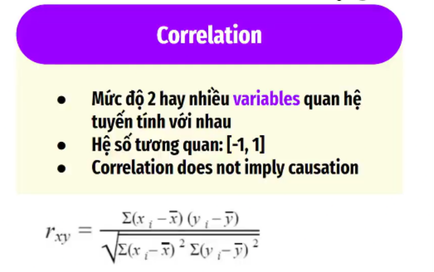
\includegraphics[width=0.8\linewidth]{15.png}
    %\fbox{\parbox[c][4cm][c]{0.8\linewidth}{\centering \textit{[Chèn ảnh: Minh họa Correlation / Multicollinearity tại đây]}}}
    \caption{Minh họa hệ số tương quan $R_{xy}$}
    \label{fig:correlation}
\end{figure}

\subsection{Correlation (Tương quan)}
\begin{itemize}
    \item Đại lượng thống kê biểu thị mức độ mà 2 hay nhiều biến thay đổi cùng nhau một cách tuyến tính.
    \item $R_{xy}$: Hệ số tương quan, có miền giá trị $R_{xy} \in [-1, 1]$:
    \begin{itemize}
        \item $R_{xy} > 0$: Tương quan dương (2 biến cùng tăng hoặc cùng giảm).
        \item $R_{xy} < 0$: Tương quan âm (1 biến tăng, 1 biến giảm).
        \item $R_{xy} = 1$: Tương quan dương hoàn hảo.
        \item $R_{xy} = -1$: Tương quan âm hoàn hảo.
        \item $R_{xy} = 0$: Hai biến không có quan hệ tuyến tính với nhau (nhưng \textbf{không thể} kết luận chúng độc lập).
    \end{itemize}
    \item Hệ số tương quan cho biết mức độ tương quan hay mối quan hệ bậc 1 (tuyến tính) giữa hai biến với nhau.
    \item Tương quan mạnh hay yếu phụ thuộc vào độ lớn của giá trị ($|R_{xy}|$ càng lớn thì các điểm dữ liệu càng nằm gần đường phù hợp nhất).
    \item \textbf{Lưu ý:} Hệ số tương quan \textbf{không thể} suy ra quan hệ nhân quả.
\end{itemize}

\subsection{(Multi)collinearity (Cộng tuyến / Đa cộng tuyến)}
\begin{itemize}
    \item Là mối quan hệ giữa các \textbf{feature} với nhau (phạm vi hẹp hơn correlation).
    \item Trong bài toán:
    \begin{itemize}
        \item \textbf{Feature:} Independent variable (biến độc lập).
        \item \textbf{Target:} Dependent variable (biến phụ thuộc, giống kiểu outcome / kết luận đầu ra).
    \end{itemize}
    \item Đa cộng tuyến là hiện tượng có lúc cần loại bỏ, có lúc không cần.
    \item Phát hiện đa cộng tuyến bằng cách tính hệ số tương quan giữa các feature.
    \item \textbf{Mục tiêu mong muốn:}
    \begin{itemize}
        \item Đối với \textbf{target và feature}: Mong muốn hệ số tương quan \textbf{càng cao càng tốt}.
        \item Đối với \textbf{các feature với nhau} (đa cộng tuyến): Mong muốn hệ số tương quan \textbf{càng thấp càng tốt} $\Rightarrow$ Càng thấp thì target càng được tác động từ nhiều hướng độc lập.
    \end{itemize}
\end{itemize}

% ==========================================
% SECTION 4: XỬ LÝ DỮ LIỆU MẤT CÂN BẰNG
% ==========================================
\section{Balance Data (Xử lý dữ liệu mất cân bằng)}

\begin{figure}[H]
    \centering
    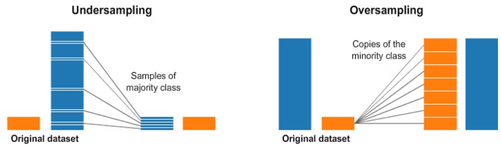
\includegraphics[width=0.8\linewidth]{16.png}
    %\fbox{\parbox[c][4cm][c]{0.8\linewidth}{\centering \textit{[Chèn ảnh: Minh họa Over-sampling (SMOTE / ADASYN) tại đây]}}}
    \caption{Các kỹ thuật cân bằng dữ liệu}
    \label{fig:balance_data}
\end{figure}

\begin{itemize}
    \item Mục đích: Làm cho dữ liệu đỡ bị mất cân bằng giữa các lớp.
    \item \textbf{Over-sampling:} Tăng mức độ tiếp xúc với phần dữ liệu thiểu số:
    \begin{itemize}
        \item \textbf{Nhân bản hóa (RandomOverSampler):} Nhân bản các thành phần thiểu số $\rightarrow$ số lượng tăng lên nhưng độ đa dạng không đổi.
        \item \textbf{Tổng hợp (SMOTE và ADASYN):}
        \begin{itemize}
            \item \textbf{SMOTE} (\textit{Synthetic Minority Oversampling Technique}): Hoạt động bằng cách chọn các điểm thuộc nhóm thiểu số gần điểm ban đầu, nội suy ra đường thẳng nối từ điểm $A$ đến điểm $B$ và chọn ngẫu nhiên một điểm nằm trên đường thẳng đó (trọng số của điểm mới dựa trên sự nội suy giữa $A$ và $B$).
            \item \textbf{ADASYN} (\textit{Adaptive Synthetic Sampling}): Hoạt động dựa trên việc sinh ra điểm nhân tạo từ các \textbf{điểm khó học} (điểm khó học là điểm bị bao quanh bởi nhiều điểm thuộc nhóm đa số $\rightarrow$ tính trọng số dựa trên các điểm đa số xung quanh, trọng số càng cao thì càng khó học; sau đó tiếp tục dùng kỹ thuật tương tự SMOTE để sinh ra điểm thiểu số nhân tạo).
        \end{itemize}
    \end{itemize}
    \item \textbf{Under-sampling:} Làm giảm phần dữ liệu đa số.
    \item $\rightarrow$ \textbf{Kết luận:} Chuộng \textbf{Over-sampling} hơn thay vì Under-sampling vì dữ liệu luôn cần được bảo toàn thay vì làm mất đi như Under-sampling.
\end{itemize}

% ==========================================
% SECTION 5: TRỰC QUAN HÓA DỮ LIỆU TRONG PYTHON
% ==========================================
\section{Data Visualization trong Python}

\begin{figure}[H]
    \centering
    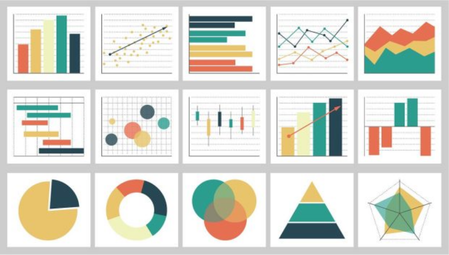
\includegraphics[width=0.8\linewidth]{17.png}
    %\fbox{\parbox[c][4cm][c]{0.8\linewidth}{\centering \textit{[Chèn ảnh: Các loại biểu đồ trực quan hóa dữ liệu tại đây]}}}
    \caption{Phân loại các biểu đồ trực quan hóa dữ liệu}
    \label{fig:data_vis}
\end{figure}

\begin{itemize}
    \item \textbf{Các thư viện phổ biến:} \texttt{numpy}, \texttt{matplotlib}, \texttt{pandas}, \texttt{seaborn}.
    \item \textbf{Các loại biểu đồ thường dùng:}
    \begin{itemize}
        \item Histogram
        \item Density plot (biểu diễn phân phối liên tục)
        \item Box plot
        \item Correlation matrix plot
        \item Scatter matrix plot
    \end{itemize}
    \item \textbf{Một số thành phần trong Matplotlib:}
    \begin{itemize}
        \item \texttt{grid}: Dóng cột và hàng (lưới tọa độ).
        \item \texttt{legend}: Chú thích (hữu ích khi một đồ thị có nhiều đường).
    \end{itemize}
\end{itemize}
\chapter{Các thuật toán Supervised Learning}

% ==========================================
% SECTION 1: TỔNG QUAN
% ==========================================
\section{Phân loại thuật toán Supervised Learning}

\begin{itemize}
    \item \textbf{Regression (Hồi quy):}
    \begin{itemize}
        \item Linear Regression (Hồi quy tuyến tính)
        \item Polynomial Regression (Hồi quy đa thức)
    \end{itemize}
    \item \textbf{Classification (Phân loại):}
    \begin{itemize}
        \item Logistic Regression
        \item Support Vector Machine (SVM)
        \item K-Nearest Neighbors (KNN)
        \item Naive Bayes
        \item Decision Tree
        \item Random Forest
    \end{itemize}
    \item $\rightarrow$ \textbf{Lưu ý về Naive Bayes:} Giả định các cột dữ liệu (feature) hoàn toàn độc lập với nhau (khó xảy ra trong thực tế vì các cột dữ liệu thường có mối quan hệ với nhau).
\end{itemize}

% ==========================================
% SECTION 2: LINEAR REGRESSION
% ==========================================
\section{Linear Regression (Hồi quy tuyến tính)}

\begin{figure}[H]
    \centering
    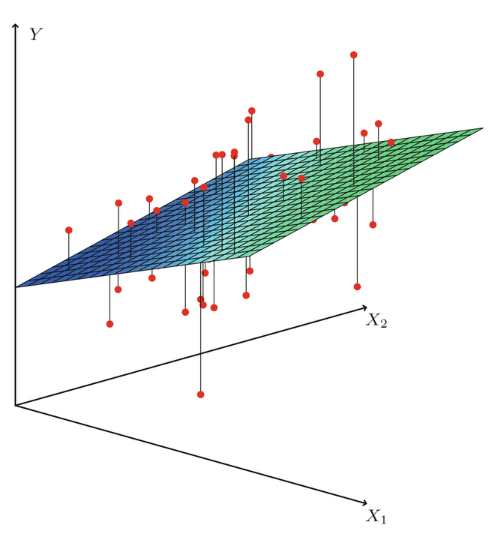
\includegraphics[width=0.8\linewidth]{21.png}
    %\fbox{\parbox[c][4cm][c]{0.8\linewidth}{\centering \textit{[Chèn ảnh: Minh họa Linear Regression tại đây]}}}
    \caption{Minh họa mô hình Linear Regression}
    \label{fig:linear_reg}
\end{figure}

\begin{itemize}
    \item Tìm đường thẳng tốt nhất sao cho tổng khoảng cách từ các điểm dữ liệu đến đường thẳng đó là bé nhất. Khi mở rộng ra không gian $n$ chiều ($n > 3$), đường thẳng trở thành \textbf{siêu phẳng (hyperplane)}.
    \item Là mô hình bậc 1.
    \item Phù hợp với dataset tuyến tính, có mối quan hệ tuyến tính giữa feature và target.
    \item Biểu diễn dạng vector: $\mathbf{x} = [x_1, x_2, x_3]^T$ là vector đầu vào (input).
    \item Tìm nghiệm để tối ưu hàm mất mát $L$.
    \item \textbf{Hạn chế của Linear Regression:}
    \begin{itemize}
        \item Nhạy cảm với nhiễu (outlier).
        \item Không biểu diễn được các mô hình phức tạp.
    \end{itemize}
\end{itemize}

% ==========================================
% SECTION 3: POLYNOMIAL REGRESSION
% ==========================================
\section{Polynomial Regression (Hồi quy đa thức)}

\begin{figure}[H]
    \centering
    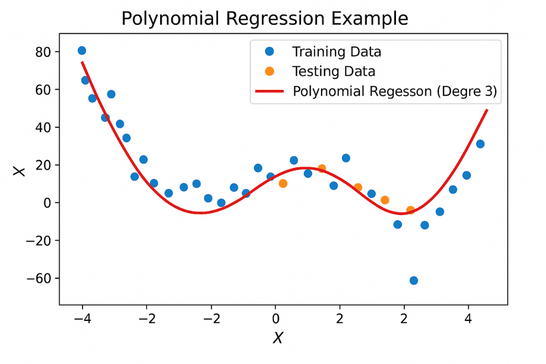
\includegraphics[width=0.8\linewidth]{22.png}
    %\fbox{\parbox[c][4cm][c]{0.8\linewidth}{\centering \textit{[Chèn ảnh: Minh họa Polynomial Regression tại đây]}}}
    \caption{Minh họa mô hình Polynomial Regression}
    \label{fig:poly_reg}
\end{figure}

\begin{itemize}
    \item Là mô hình có bậc lớn hơn 1.
    \item Cho khả năng dự đoán tốt hơn trên dữ liệu phi tuyến tính, nhưng đồng thời cũng \textbf{dễ bị Overfitting} hơn.
\end{itemize}

% ==========================================
% SECTION 4: LOGISTIC REGRESSION
% ==========================================
\section{Logistic Regression}

\begin{figure}[H]
    \centering
    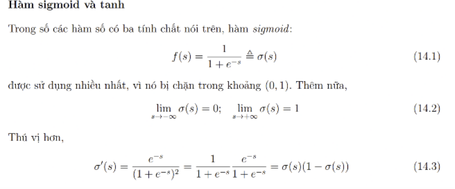
\includegraphics[width=0.8\linewidth]{23.png}
    %\fbox{\parbox[c][4cm][c]{0.8\linewidth}{\centering \textit{[Chèn ảnh: Hàm Sigmoid và Logistic Regression tại đây]}}}
    \caption{Hàm Sigmoid trong Logistic Regression}
    \label{fig:logistic_reg}
\end{figure}

\begin{itemize}
    \item Sử dụng \textbf{hàm Sigmoid} để chuyển đầu ra (output) về thang đo $[0, 1]$.
    \item Chia đoạn để phân lớp, ví dụ: $[0, 0.5] \rightarrow \text{Class 1}$, $(0.5, 1] \rightarrow \text{Class 2}$.
    \item \textbf{Threshold (Ngưỡng):} Điểm phân định ranh giới, điểm kích hoạt để chuyển đổi từ trạng thái (class) này sang trạng thái khác.
\end{itemize}
\begin{figure}[H]
    \centering
    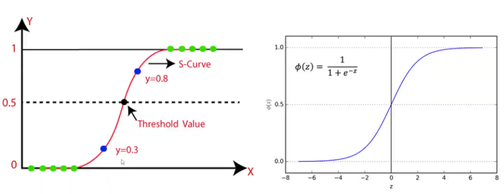
\includegraphics[width=0.8\linewidth]{24.png}
    %\fbox{\parbox[c][4cm][c]{0.8\linewidth}{\centering \textit{[Chèn ảnh: Hàm Sigmoid và Logistic Regression tại đây]}}}
    \caption{Hàm Sigmoid trong Logistic Regression}
    \label{fig:logistic_reg2}
\end{figure}

% ==========================================
% SECTION 5: SUPPORT VECTOR MACHINE (SVM)
% ==========================================
\section{Support Vector Machine (SVM)}

\begin{figure}[H]
    \centering
    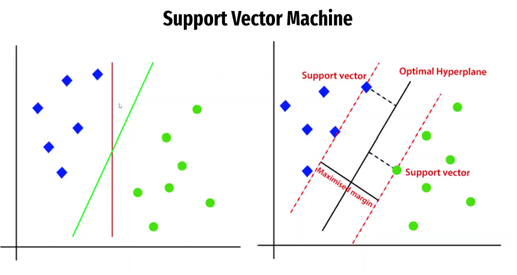
\includegraphics[width=0.8\linewidth]{25.png}
    %\fbox{\parbox[c][4cm][c]{0.8\linewidth}{\centering \textit{[Chèn ảnh: Minh họa Support Vector và Margin tại đây]}}}
    \caption{Nguyên lý hoạt động của Support Vector Machine}
    \label{fig:svm}
\end{figure}


\begin{itemize}
    \item Tập trung vào các điểm dữ liệu nằm trên ranh giới để phân định chúng, từ đó tạo ra đường/vector phân cách giữa các class. Thay vì fit toàn bộ các điểm dữ liệu, SVM chỉ xử lý các điểm dễ phân loại sai.
    \item \textbf{Support Vector:} Là những điểm dễ sai nhất vì chúng nằm sát đường phân cách.
    \item \textbf{Hai điều kiện để chọn đường phân cách tối ưu:}
    \begin{itemize}
        \item Khoảng cách từ hai điểm gần nhất của hai miền đến đường phân cách phải \textbf{bằng nhau}.
        \item Phải tạo ra được \textbf{khoảng cách (margin) tối đa} giữa Support Vector và đường phân cách.
    \end{itemize}
    \item $\rightarrow$ \textbf{Xử lý dữ liệu thực tế (Not Linearly Separable):}
    \begin{itemize}
        \item Khi dữ liệu không thể tách tuyến tính trong không gian hiện tại, SVM sẽ thêm chiều mới vào (chiều mới là tổ hợp của các chiều cũ $\rightarrow$ tạo thêm nhiều feature mới).
        \item Tiếp tục thêm chiều mới cho đến khi có thể phân chia được các lớp.
    \end{itemize}
\end{itemize}
\begin{figure}[H]
    \centering
    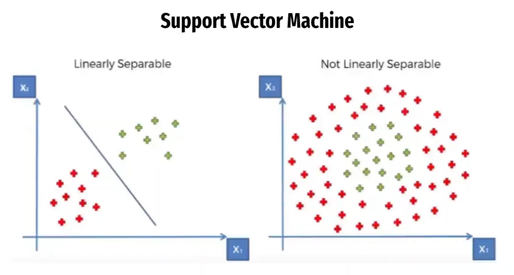
\includegraphics[width=0.8\linewidth]{26.png}
    %\fbox{\parbox[c][4cm][c]{0.8\linewidth}{\centering \textit{[Chèn ảnh: Minh họa Support Vector và Margin tại đây]}}}
    \caption{minh họa}
    \label{fig:svm1}
\end{figure}

\begin{figure}[H]
    \centering
    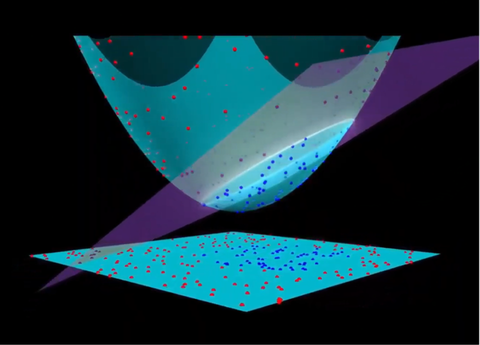
\includegraphics[width=0.8\linewidth]{27.png}
    %\fbox{\parbox[c][4cm][c]{0.8\linewidth}{\centering \textit{[Chèn ảnh: Minh họa Support Vector và Margin tại đây]}}}
    \caption{minh họa}
    \label{fig:svm2}
\end{figure}

\begin{figure}[H]
    \centering
    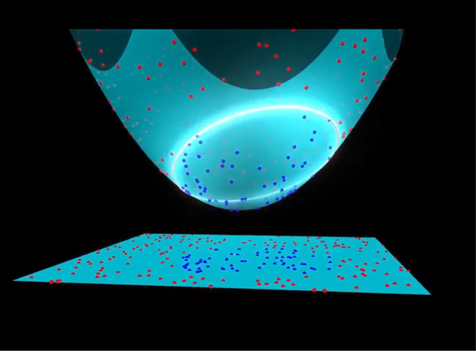
\includegraphics[width=0.8\linewidth]{28.png}
    %\fbox{\parbox[c][4cm][c]{0.8\linewidth}{\centering \textit{[Chèn ảnh: Minh họa Support Vector và Margin tại đây]}}}
    \caption{minh họa}
    \label{fig:svm3}
\end{figure}

\begin{figure}[H]
    \centering
    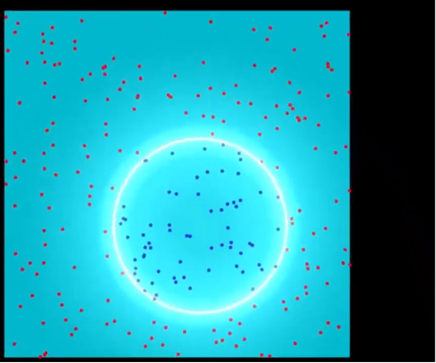
\includegraphics[width=0.8\linewidth]{29.png}
    %\fbox{\parbox[c][4cm][c]{0.8\linewidth}{\centering \textit{[Chèn ảnh: Minh họa Support Vector và Margin tại đây]}}}
    \caption{minh họa}
    \label{fig:svm4}
\end{figure}

\begin{figure}[H]
    \centering
    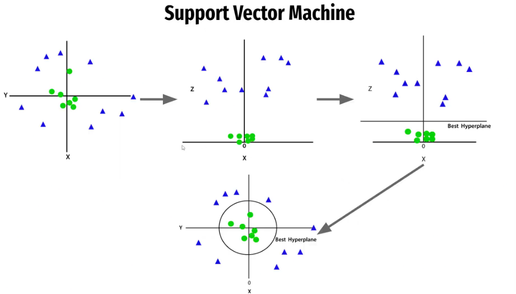
\includegraphics[width=0.8\linewidth]{30.png}
    %\fbox{\parbox[c][4cm][c]{0.8\linewidth}{\centering \textit{[Chèn ảnh: Minh họa Support Vector và Margin tại đây]}}}
    \caption{minh họa}
    \label{fig:svm5}
\end{figure}
% ==========================================
% SECTION 6: K-NEAREST NEIGHBORS (KNN)
% ==========================================
\section{K-Nearest Neighbors (KNN)}

\begin{figure}[H]
    \centering
    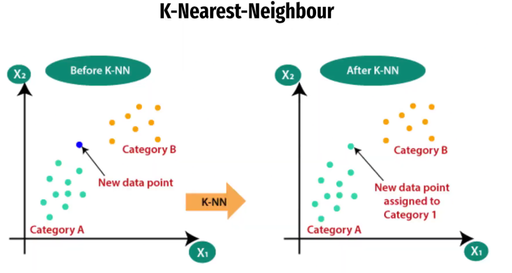
\includegraphics[width=0.8\linewidth]{31.png}
    %\fbox{\parbox[c][4cm][c]{0.8\linewidth}{\centering \textit{[Chèn ảnh: Minh họa thuật toán KNN tại đây]}}}
    \caption{Nguyên lý phân loại của K-Nearest Neighbors}
    \label{fig:knn}
\end{figure}

\begin{itemize}
    \item Khi có một điểm dữ liệu mới cần phân loại, thuật toán sẽ chọn ra $K$ điểm gần nó nhất rồi xét xem class nào chiếm đa số thì gán điểm mới vào class đó.
    \item \textbf{Tính khoảng cách:} Vì dựa vào độ gần, các feature bắt buộc phải được chuẩn hóa để phạm vi (range) của từng feature công bằng với nhau, tránh việc giá trị lớn của một feature áp đảo các feature khác.
    \item Thường chọn $K$ là \textbf{số lẻ} (để tránh hòa phiếu), không nên chọn $K$ quá bé hoặc quá lớn.
    \item \textbf{Đặc điểm:} Thời gian huấn luyện $\text{Training} = 0$; quá trình tính toán chỉ thực sự diễn ra lúc thực thi (dự đoán).
\end{itemize}

% ==========================================
% SECTION 7: DECISION TREE
% ==========================================
\section{Decision Tree (Cây quyết định)}

\begin{figure}[H]
    \centering
    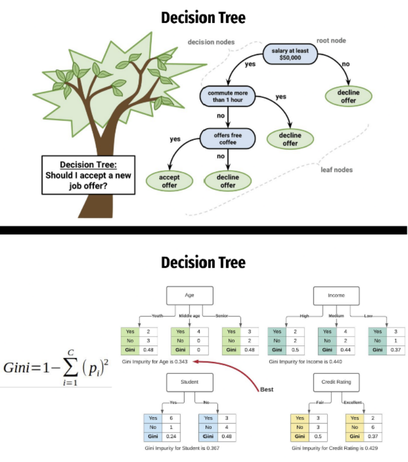
\includegraphics[width=0.8\linewidth]{32.png}
    %\fbox{\parbox[c][4cm][c]{0.8\linewidth}{\centering \textit{[Chèn ảnh: Cấu trúc Decision Tree tại đây]}}}
    \caption{Cấu trúc của một Decision Tree}
    \label{fig:decision_tree}
\end{figure}

\begin{itemize}
    \item \textbf{Các thành phần chính:}
    \begin{itemize}
        \item \textbf{Decision Nodes:} Các nút quyết định (nơi rẽ nhánh theo điều kiện).
        \item \textbf{Leaf Nodes:} Các nút lá (chứa kết quả phân loại/dự đoán cuối cùng).
    \end{itemize}
    \item \textbf{Gini Index (Gini Impurity):} Chỉ số dùng để tính toán và chọn feature làm nút gốc (root) cho các cây con. Giá trị càng gần $0$ càng tốt (thuần khiết), càng gần $0.5$ càng tồi (hỗn tạp).
    \item \textbf{Ưu điểm:}
    \begin{itemize}
        \item Có thể giải quyết tốt các bài toán phi tuyến tính.
        \item Làm việc với không gian nhiều chiều (nhiều feature) với độ chính xác cao.
        \item Rất trực quan và dễ dàng giải thích kết quả.
    \end{itemize}
\end{itemize}

% ==========================================
% SECTION 8: RANDOM FOREST
% ==========================================
\section{Random Forest}

\begin{figure}[H]
    \centering
    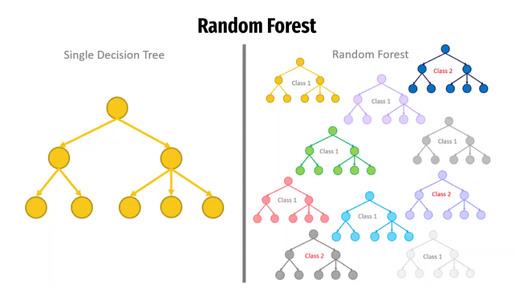
\includegraphics[width=0.8\linewidth]{33.png}
    %\fbox{\parbox[c][4cm][c]{0.8\linewidth}{\centering \textit{[Chèn ảnh: Mô hình Random Forest tại đây]}}}
    \caption{Cơ chế kết hợp nhiều cây trong Random Forest}
    \label{fig:random_forest}
\end{figure}
\begin{figure}[H]
    \centering
    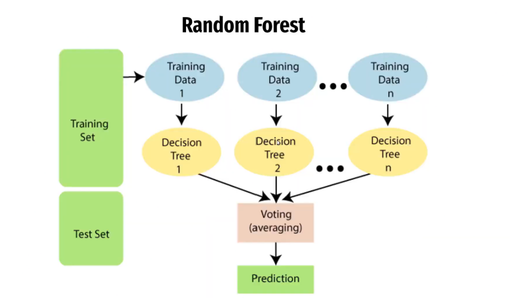
\includegraphics[width=0.8\linewidth]{34.png}
    %\fbox{\parbox[c][4cm][c]{0.8\linewidth}{\centering \textit{[Chèn ảnh: Mô hình Random Forest tại đây]}}}
    \caption{Cơ chế kết hợp nhiều cây trong Random Forest}
    \label{fig:random_forest1}
\end{figure}

\begin{itemize}
    \item Không huấn luyện toàn bộ các cây trên toàn bộ tập dữ liệu, mà chia nhỏ bộ dataset và chọn ngẫu nhiên một tập con các feature cho từng cây.
    \item Cho độ tin cậy cao hơn và giảm overfitting tốt hơn so với một cây Decision Tree đơn lẻ.
\end{itemize}
\chapter{Các thuật toán Unsupervised Learning}

% ==========================================
% SECTION 1: K-MEANS CLUSTERING
% ==========================================
\section{K-Means Clustering}

\begin{figure}[H]
    \centering
    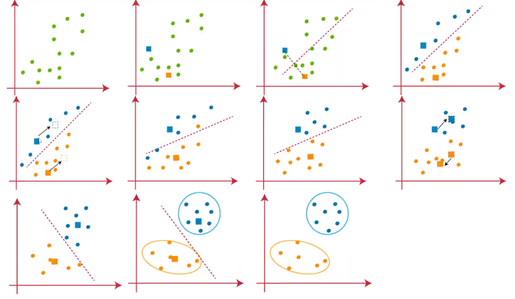
\includegraphics[width=0.8\linewidth]{41.png}
    %\fbox{\parbox[c][4cm][c]{0.8\linewidth}{\centering \textit{[Chèn ảnh: Minh họa thuật toán K-Means Clustering tại đây]}}}
    \caption{Nguyên lý phân cụm của thuật toán K-Means Clustering}
    \label{fig:kmeans}
\end{figure}

\begin{itemize}
    \item Liên tục lặp lại hành động chọn tâm cụm (center/centroid) và cập nhật lại vị trí tâm dựa trên giá trị trung bình của các điểm dữ liệu thuộc nhóm đã phân chia trước đó.
    \item Quá trình này được lặp đi lặp lại cho đến khi hội tụ — tức là khi vị trí của các tâm cụm không còn thay đổi nữa.
\end{itemize}
\chapter{Phương thức chia dữ liệu}

% ==========================================
% SECTION 1: K-FOLD CROSS VALIDATION
% ==========================================
\section{K-Fold Cross Validation}

\begin{figure}[H]
    \centering
    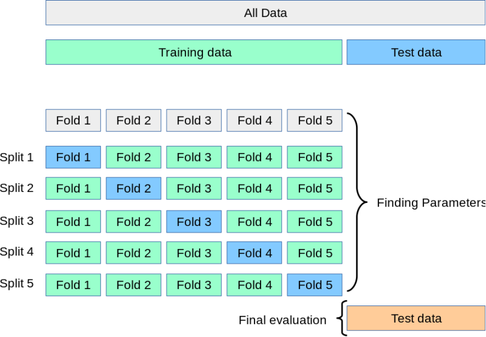
\includegraphics[width=0.8\linewidth]{51.png}
    %\fbox{\parbox[c][4cm][c]{0.8\linewidth}{\centering \textit{[Chèn ảnh: Minh họa K-Fold Cross Validation tại đây]}}}
    \caption{Cơ chế phân chia dữ liệu trong K-Fold Cross Validation}
    \label{fig:kfold_cv}
\end{figure}

\begin{itemize}
    \item \textbf{Mục đích:} Cách chia và tận dụng toàn bộ dữ liệu huấn luyện để đánh giá mô hình một cách khách quan và toàn diện hơn.
    \item \textbf{Test set:} Được tách riêng ra khỏi bộ dữ liệu ban đầu (\textit{unseen data} — không tham gia vào quá trình huấn luyện).
    \item \textbf{Quá trình huấn luyện:} Phần dữ liệu train được chia thành $K$ phần (folds) bằng nhau và thực hiện huấn luyện mô hình $K$ lần. Ở mỗi lần chạy:
    \begin{itemize}
        \item Chọn $1$ phần làm tập \textbf{Validation}.
        \item Chọn $K - 1$ phần còn lại làm tập \textbf{Train}.
    \end{itemize}
    \item \textbf{Đánh giá cuối cùng:} Kết quả đánh giá mô hình là \textbf{trung bình cộng} của tất cả các kết quả thu được sau $K$ lần huấn luyện.
\end{itemize}
\chapter{Gradient Descent và các biến thể}

% ==========================================
% SECTION 1: BÀI TOÁN
% ==========================================
\section{Bài toán tối ưu}
\begin{itemize}
    \item Xuất phát từ một điểm được coi là gần với nghiệm của bài toán, sau đó dùng phép toán lặp để tiến dần đến nghiệm cần tìm.
\end{itemize}

% ==========================================
% SECTION 2: GD CHO HÀM MỘT BIẾN
% ==========================================
\section{Gradient Descent cho hàm một biến}

\begin{figure}[H]
    \centering
    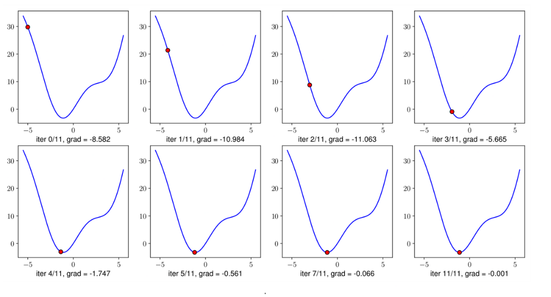
\includegraphics[width=0.8\linewidth]{61.png}
    %\fbox{\parbox[c][4cm][c]{0.8\linewidth}{\centering \textit{[Chèn ảnh: Minh họa Gradient Descent cho hàm 1 biến tại đây]}}}
    \caption{Cơ chế cập nhật điểm trong Gradient Descent một biến}
    \label{fig:gd_1d}
\end{figure}

\begin{itemize}
    \item \textbf{Công thức cập nhật:}
    \[
        x_{t+1} = x_t - \eta f'(x_t)
    \]
    trong đó $\eta$ là \textit{learning rate} (tốc độ học).
    \item Đi ngược hướng đạo hàm ($-f'(x_t)$) để tìm điểm có giá trị hàm mất mát nhỏ hơn.
    \item Mục tiêu là đưa $x$ về vị trí tối ưu $x^*$, nhưng ta không biết $x^*$ từ trước mà hoàn toàn phải tính toán dựa trên độ dốc hiện tại và tốc độ học.
    \item \textbf{Vai trò của đạo hàm $f'(x_t)$:} Chỉ rõ hướng và độ lớn của độ dốc, giúp tự động điều chỉnh bước nhảy:
    \begin{itemize}
        \item Khi còn xa đáy (điểm ở vị trí cao): độ dốc lớn $\rightarrow$ bước nhảy lớn để tiết kiệm thời gian.
        \item Càng gần về \textit{global minimum}: độ dốc nhỏ dần $\rightarrow$ bước nhảy nhỏ để tiến đến cực tiểu một cách thận trọng và chính xác hơn.
    \end{itemize}
    \item \textbf{Vai trò của Learning rate ($\eta$):} Thể hiện độ lớn bước nhảy / tốc độ di chuyển của điểm.
    \item Tốc độ hội tụ của Gradient Descent phụ thuộc vào cả \textbf{điểm xuất phát} và \textbf{learning rate}.
\end{itemize}

\begin{figure}[H]
    \centering
    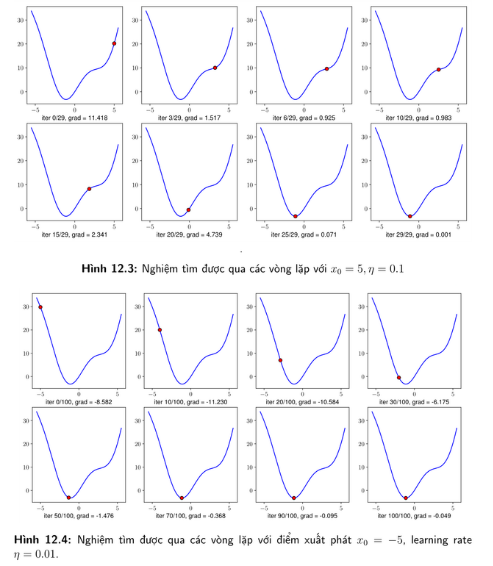
\includegraphics[width=0.8\linewidth]{62.png}
    %\fbox{\parbox[c][4cm][c]{0.8\linewidth}{\centering \textit{[Chèn ảnh: Minh họa Gradient Descent cho hàm 1 biến tại đây]}}}
    \caption{Cơ chế cập nhật điểm trong Gradient Descent một biến}
    \label{fig:gd_1d1}
\end{figure}

\begin{figure}[H]
    \centering
    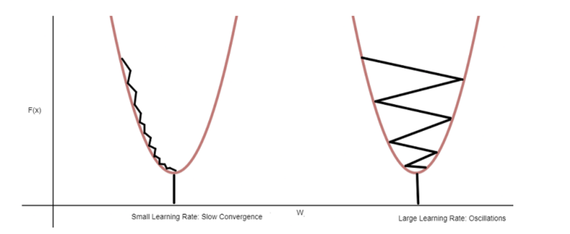
\includegraphics[width=0.8\linewidth]{64.png}
    %\fbox{\parbox[c][4cm][c]{0.8\linewidth}{\centering \textit{[Chèn ảnh: Minh họa Gradient Descent cho hàm 1 biến tại đây]}}}
    \caption{Cơ chế cập nhật điểm trong Gradient Descent một biến}
    \label{fig:gd_1d2}
\end{figure}
% ==========================================
% SECTION 3: GD CHO HÀM NHIỀU BIẾN
% ==========================================
\section{Gradient Descent cho hàm nhiều biến}

\begin{itemize}
    \item Là sự mở rộng trực tiếp từ trường hợp hàm một biến.
    \item Chuyển từ đạo hàm lên Gradient.
    \item Gradient: Tập hợp tất cả các đạo hàm riêng.
    \item \textbf{Biểu thức cập nhật:}
    \[
        \theta_{t+1} = \theta_t - \eta \nabla_\theta f(\theta_t)
    \]
\end{itemize}

% ==========================================
% SECTION 4: MOMENTUM
% ==========================================
\section{Gradient Descent với Momentum}

\begin{figure}[H]
    \centering
    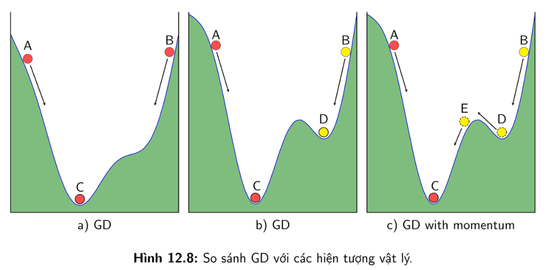
\includegraphics[width=0.8\linewidth]{65.png}
    %\fbox{\parbox[c][4cm][c]{0.8\linewidth}{\centering \textit{[Chèn ảnh: Minh họa Gradient Descent với Momentum tại đây]}}}
    \caption{Gradient Descent kết hợp Momentum vượt qua cực tiểu địa phương}
    \label{fig:gd_momentum}
\end{figure}

\begin{itemize}
    \item \textbf{Mục đích:} Giúp Gradient Descent thông thường thoát khỏi cực tiểu địa phương (\textit{local minimum}).
    \item \textbf{Ý tưởng:} Bổ sung thêm thành phần động lượng (xuất phát từ cơ học/động lực học) vào GD thông thường.
    \item \textbf{Công thức:}
    \[
        v_t = \gamma v_{t-1} + \eta \nabla_\theta J(\theta_t), \qquad \theta_{t+1} = \theta_t - v_t
    \]
    thực chất $v_t$ là một biến tích lũy (vận tốc).
    \item \textbf{Cơ chế triệt tiêu (giảm zigzag):} Nếu ở bước hiện tại điểm bị nhảy sang sườn dốc bên kia, hệ số $\gamma$ (thường chọn $\gamma = 0.9$) và $v_{t-1}$ sẽ giúp triệt tiêu thành phần dao động, làm $v_t$ nhỏ lại và hạn chế hiện tượng nhảy qua lại (zigzag).
    \item $v_t$ cộng dồn là một chuỗi hội tụ về $0$; khi đến đích vẫn có thể xảy ra một số lần đung đưa trước khi dừng hẳn.
    \item \textbf{Các trạng thái của $v_t$:}
    \begin{itemize}
        \item Lúc đầu ở trên đỉnh cao (độ dốc lớn), $v_t$ sẽ liên tục tăng tốc.
        \item $v_t$ bắt đầu giảm ngay khi lượng tăng thêm nhỏ hơn lượng thất thoát: $\eta \nabla_\theta J(\theta_t) < (1 - \gamma) v_{t-1}$.
        \item Đến một thời điểm khi $v_{t-1}$ quá lớn trong khi dốc thoải dần, $10\%$ thất thoát trở thành một con số lớn khiến lượng tăng thêm từ độ dốc không thể bù nổi vào.
    \end{itemize}
    \item \textbf{Nhược điểm:} Hiện tượng \textbf{Overshooting} (vượt quá đích do quán tính lớn).
\end{itemize}

% ==========================================
% SECTION 5: NESTEROV ACCELERATED GRADIENT (NAG)
% ==========================================
\section{Nesterov Accelerated Gradient (NAG)}

\begin{figure}[H]
    \centering
    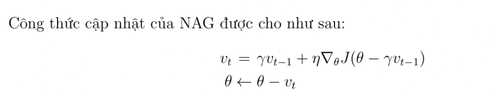
\includegraphics[width=0.8\linewidth]{67.png}
    %\fbox{\parbox[c][4cm][c]{0.8\linewidth}{\centering \textit{[Chèn ảnh: So sánh Momentum và Nesterov Accelerated Gradient tại đây]}}}
    \caption{Công thức cập nhật}
    \label{fig:gd_nag}
\end{figure}

\begin{itemize}
    \item \textbf{Mục đích chính:} Hạn chế hiện tượng \textit{overshooting} của Momentum.
    \item \textbf{Ý tưởng chính:} Dự đoán trước vị trí của nghiệm một bước.
    \item \textbf{Sự khác biệt giữa Momentum và NAG (nằm ở điểm lấy đạo hàm):}
    \begin{itemize}
        \item \textbf{Momentum:} Lấy đạo hàm tại vị trí hiện tại $\theta_t$ (kết hợp giữa momentum vector và gradient tại thời điểm hiện tại).
        \item \textbf{NAG:} Điểm lấy đạo hàm là vị trí dự đoán tiếp theo nếu đi theo momentum: $\theta_t - \gamma v_{t-1}$ (kết hợp giữa momentum vector và gradient tại vị trí dự đoán).
    \end{itemize}
    \item Nhờ đoán trước vị trí tiếp theo, NAG có cơ chế phanh/triệt tiêu mạnh hơn khi sắp vượt quá đích.
\end{itemize}

\begin{figure}[H]
    \centering
    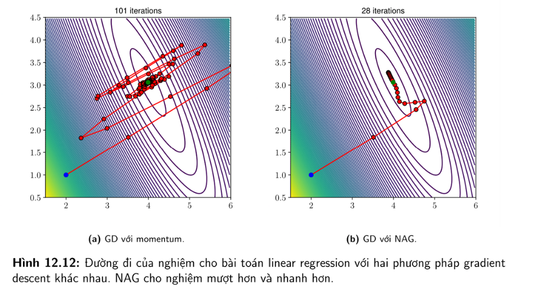
\includegraphics[width=0.8\linewidth]{68.png}
    %\fbox{\parbox[c][4cm][c]{0.8\linewidth}{\centering \textit{[Chèn ảnh: So sánh Momentum và Nesterov Accelerated Gradient tại đây]}}}
    \label{fig:gd_nag1}
\end{figure}

% ==========================================
% SECTION 6: BATCH, STOCHASTIC & MINI-BATCH GD
% ==========================================
\section{Các biến thể theo lượng dữ liệu cập nhật}

\subsection{Batch Gradient Descent}
\begin{itemize}
    \item Các thuật toán được đề cập ở các mục trước thuộc nhóm \textbf{Batch GD}.
    \item Khi cập nhật tham số $\theta$, thuật toán sử dụng \textbf{toàn bộ} các điểm dữ liệu $x_i$.
    \item \textbf{Hạn chế:} Với cơ sở dữ liệu lớn, việc tính toán trên toàn bộ dữ liệu cho mỗi bước cập nhật tốn rất nhiều thời gian.
\end{itemize}

\subsection{Stochastic Gradient Descent (SGD)}
\begin{itemize}
    \item Chấp nhận sai sót nhất định để đổi lấy hiệu quả tính toán cao.
    \item Tính đạo hàm tại \textbf{một điểm hoàn toàn ngẫu nhiên} rồi cập nhật tham số luôn, thay vì tính tại tất cả mọi điểm rồi lấy trung bình như GD nguyên thủy.
    \item Đạo hàm tại một điểm ngẫu nhiên được kỳ vọng là khá gần với đạo hàm trung bình của hàm mất mát trên toàn bộ dữ liệu.
    \item \textbf{Số lần cập nhật sau 1 epoch:} Là $N$ lần (so với GD nguyên thủy chỉ là $1$ lần). Tập dữ liệu được xáo trộn (shuffle) trước mỗi epoch.
    \item Để tránh hiện tượng dao động lặp lại quá nhiều quanh cực tiểu, SGD thường kết hợp với kỹ thuật \textbf{Learning Rate Decay} (giảm dần tốc độ học theo thời gian).
\end{itemize}

\subsection{Mini-batch Gradient Descent}
\begin{itemize}
    \item Kết hợp và tối ưu giữa Batch GD nguyên thủy (quá chậm) và SGD (quá nhiễu).
    \item Chia tập dữ liệu lớn ($N$ phần tử) thành nhiều tập nhỏ (mỗi tập có $k$ phần tử), tính toán và cập nhật tham số trên từng tập nhỏ đó $\rightarrow$ một epoch có $N/k$ lần cập nhật.
    \item \textbf{Ưu điểm:} Giảm thiểu sai sót/nhiễu của SGD và tăng tốc độ, số lần cập nhật so với Batch GD.
\end{itemize}

\begin{figure}[H]
    \centering
    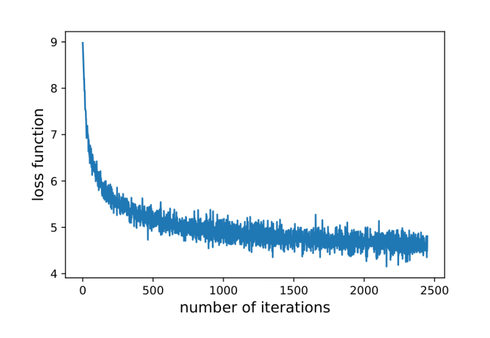
\includegraphics[width=0.8\linewidth]{69.png}
    %\fbox{\parbox[c][4cm][c]{0.8\linewidth}{\centering \textit{[Chèn ảnh: So sánh Momentum và Nesterov Accelerated Gradient tại đây]}}}
    \caption{Mini-batch visualization}
    \label{fig:mnb_visualization}
\end{figure}


\begin{figure}[H]
    \centering
    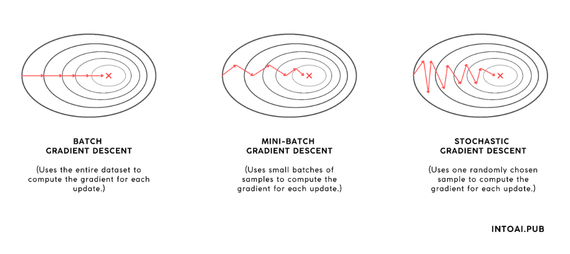
\includegraphics[width=0.8\linewidth]{610.png}
    %\fbox{\parbox[c][4cm][c]{0.8\linewidth}{\centering \textit{[Chèn ảnh: So sánh Momentum và Nesterov Accelerated Gradient tại đây]}}}
    \caption{Tương quan giữa các phương pháp}
    \label{fig:tuongquan}
\end{figure}

% ==========================================
% SECTION 7: THỜI ĐIỂM DỪNG THUẬT TOÁN
% ==========================================
\section{Thời điểm dừng thuật toán (Stopping Criteria)}

\begin{itemize}
    \item \textbf{Giới hạn số vòng lặp:} Đặt trước số epoch/iteration tối đa. Hạn chế là dễ dừng ở thời điểm chưa tối ưu.
    \item \textbf{So sánh gradient (độ dốc):} So sánh giá trị gradient của nghiệm giữa hai lần cập nhật liên tiếp, khi đủ nhỏ thì dừng. Hạn chế là đôi khi việc tính đạo hàm phức tạp.
    \item \textbf{So sánh giá trị hàm mất mát (độ cao):} So sánh giá trị hàm mất mát tại hai thời điểm cập nhật liên tiếp, khi độ chênh lệch đủ nhỏ thì dừng.
    \item \textbf{Early Stopping (Kiểm tra định kỳ):} Cho thuật toán chạy với số vòng lặp rất lớn; trong quá trình chạy, thường xuyên kiểm tra chất lượng mô hình trên tập huấn luyện và/hoặc tập validation để dừng đúng lúc.
\end{itemize}



% \chapter{Machine Learning Pipeline}

% ==========================================
% SECTION 1: ML PIPELINE
% ==========================================
\section{Quy trình Machine Learning (ML Pipeline)}

\begin{figure}[H]
    \centering
    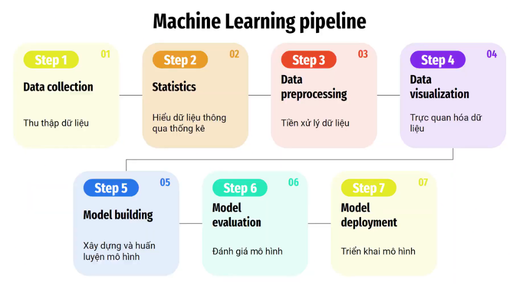
\includegraphics[width=0.8\linewidth]{11.png}
    %\fbox{\parbox[c][4cm][c]{0.8\linewidth}{\centering \textit{[Chèn ảnh: Tổng quan ML Pipeline tại đây]}}}
    \caption{Quy trình tổng quan của một ML Pipeline}
    \label{fig:ml_pipeline}
\end{figure}

\subsection{Step 1: Data Collection (Thu thập dữ liệu)}
\begin{itemize}
    \item Xác định bài toán và dữ liệu cần có.
    \item Thu thập dữ liệu.
    \item Đánh nhãn (Annotation).
    \item \textbf{OUTPUT:} Dữ liệu thô (Raw data).
\end{itemize}

\subsection{Step 2: Statistics (Thống kê mô tả)}
\begin{itemize}
    \item Thống kê: Tính toán các thông số cơ bản:
    \begin{itemize}
        \item \textbf{Mean:} Trung bình.
        \item \textbf{Median:} Trung vị.
        \item \textbf{Std:} Độ lệch chuẩn.
        \item \textbf{Variance:} Phương sai.
        \item \textbf{Min/Max:} Giá trị nhỏ nhất / lớn nhất.
        \item \textbf{Q1, Q2, Q3:} Tứ phân vị.
        \item \textbf{Mode:} Điểm dữ liệu có tần số xuất hiện lớn nhất.
    \end{itemize}
    \item \textbf{OUTPUT:} Cung cấp cái nhìn tổng quan về bộ dữ liệu.
\end{itemize}

\subsection{Step 3: Data Preprocessing (Tiền xử lý dữ liệu)}
\begin{itemize}
    \item Đưa dữ liệu về dạng máy tính có thể hiểu được (dạng số).
    \item Làm sạch dữ liệu.
    \item Chuẩn hóa: Đưa mọi tham số về cùng một thang đo.
    \item Phân chia dữ liệu: Training set, Validation set, Test set.
    \item Tạo đặc trưng mới dựa trên dữ liệu sau xử lý.
    \item Các bước trong quá trình này được xây dựng và mô hình hóa thành một pipeline/mô hình riêng, phục vụ cho các pha khác để đảm bảo tính thống nhất.
    \item \textbf{OUTPUT:} Dữ liệu đã được làm sạch, chuẩn hóa và phân chia thành từng cụm phục vụ cho từng bước.
\end{itemize}

\subsection{Step 4: Data Visualization (Trực quan hóa dữ liệu)}
\begin{itemize}
    \item Dựa trên dữ liệu cung cấp, cần trực quan hóa dữ liệu để có thể dễ dàng quan sát.
    \item Sử dụng các thư viện của python.
    \item \textbf{OUTPUT:} Biểu đồ.
\end{itemize}

\subsection{Step 5: Model Building (Xây dựng mô hình)}
\begin{itemize}
    \item Chọn thuật toán phù hợp.
    \item Tiến hành training dựa trên Training set.
    \item \textbf{Tinh chỉnh} các tham số dựa trên kết quả đầu ra.
    \item Sử dụng thêm các mô hình khác để so sánh.
    \item \textbf{OUTPUT:} Trả về mô hình đã huấn luyện, có thể dùng để dự đoán.
\end{itemize}

\subsection{Step 6: Model Evaluation (Đánh giá mô hình)}
\begin{itemize}
    \item Từ kết quả thu được trên Test set, tính toán các thông số như: Accuracy, Precision, Recall, F1 score, ROC, AUC.
    \item Kiểm tra hiện tượng Overfitting (Train tốt, Test kém).
    \item Tiến hành đánh giá kết quả của mô hình sau bài test.
    \item \textbf{OUTPUT:} Dựa vào kết quả để kết luận mô hình có đạt không. Nếu không đạt, cần xác định quay lại bước nào để tinh chỉnh.
\end{itemize}

\subsection{Step 7: Model Deployment (Triển khai mô hình)}
\begin{itemize}
    \item Tích hợp, triển khai mô hình vào các thiết bị, cloud,... để sử dụng tùy vào mục đích.
\end{itemize}

\subsection{Lưu ý về vòng lặp của Pipeline}
\begin{figure}[H]
    \centering
    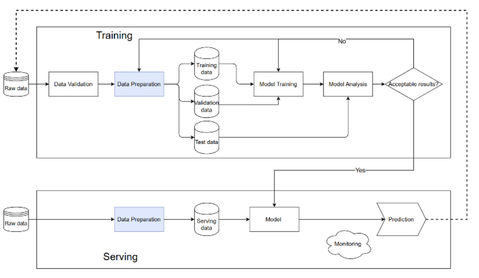
\includegraphics[width=0.8\linewidth]{12.png}
    \caption{Machine learning pipeline}
    \label{fig: hieuchinh}
\end{figure}
\begin{itemize}
    \item Pipeline thường \textbf{không chạy một chiều}, cần phải cải thiện lại nếu Step 6 chưa đạt kết quả như kỳ vọng.
    \item Đường đi phản hồi: $\text{Prediction} \rightarrow \text{Raw data}$.
    \item Nghĩa là dữ liệu thu được từ mô hình được đưa ngược về để làm Training set nhằm đảm bảo mô hình có thể bắt kịp với những thay đổi thực tế.
\end{itemize}

% ==========================================
% SECTION 2: CHI TIẾT TIỀN XỬ LÝ DỮ LIỆU
% ==========================================
\section{Các bước Tiền xử lý dữ liệu (Data Preprocessing)}

\begin{figure}[H]
    \centering
    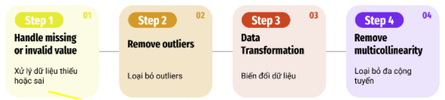
\includegraphics[width=0.8\linewidth]{13.png}
    %\fbox{\parbox[c][4cm][c]{0.8\linewidth}{\centering \textit{[Chèn ảnh: Quy trình Data Preprocessing tại đây]}}}
    \caption{Các bước chính trong tiền xử lý dữ liệu}
    \label{fig:data_preprocessing}
\end{figure}

\begin{itemize}
    \item \textbf{Step 1:} Handle missing or invalid values (Xử lý dữ liệu thiếu hoặc không hợp lệ).
    \item \textbf{Step 2:} Remove outliers (Loại bỏ các điểm ngoại lai).
    \item \textbf{Step 3:} Data transformation (Biến đổi dữ liệu):
    \begin{itemize}
        \item \textbf{Numerical feature} (Thuộc tính dạng số):
        \begin{itemize}
            \item Tiền xử lý: \texttt{MinMaxScaler} (nhạy cảm với outliers), \texttt{StandardScaler}.
            \item \textbf{Continuous:} Dữ liệu liên tục.
            \item \textbf{Discrete:} Dữ liệu rời rạc.
        \end{itemize}
        \item \textbf{Categorical feature} (Thuộc tính dạng phân loại):
        \begin{itemize}
            \item \textbf{Ordinal} (Thứ bậc) $\rightarrow$ \texttt{OrdinalEncoder}.
            \item \textbf{Nominal} (Danh nghĩa) $\rightarrow$ One-hot encoding, Hash encoding, Word Embedding.
        \end{itemize}
    \end{itemize}
    \begin{figure}[H]
    \centering
    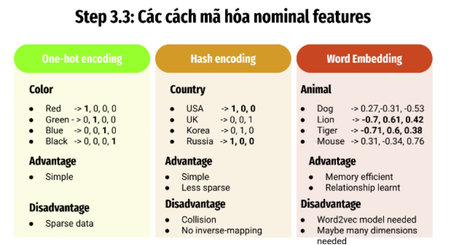
\includegraphics[width=0.8\linewidth]{14.png}
    %\fbox{\parbox[c][4cm][c]{0.8\linewidth}{\centering \textit{[Chèn ảnh: Minh họa Correlation / Multicollinearity tại đây]}}}
    \caption{Các cách mã hóa}
    \label{fig:encoder}
\end{figure}
    \item \textbf{Step 4:} Remove multicollinearity (Loại bỏ hiện tượng đa cộng tuyến).
\end{itemize}

% ==========================================
% SECTION 3: TƯƠNG QUAN & ĐA CỘNG TUYẾN
% ==========================================
\section{Mối quan hệ giữa các biến}

\begin{figure}[H]
    \centering
    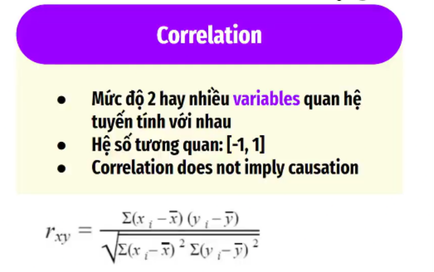
\includegraphics[width=0.8\linewidth]{15.png}
    %\fbox{\parbox[c][4cm][c]{0.8\linewidth}{\centering \textit{[Chèn ảnh: Minh họa Correlation / Multicollinearity tại đây]}}}
    \caption{Minh họa hệ số tương quan $R_{xy}$}
    \label{fig:correlation}
\end{figure}

\subsection{Correlation (Tương quan)}
\begin{itemize}
    \item Đại lượng thống kê biểu thị mức độ mà 2 hay nhiều biến thay đổi cùng nhau một cách tuyến tính.
    \item $R_{xy}$: Hệ số tương quan, có miền giá trị $R_{xy} \in [-1, 1]$:
    \begin{itemize}
        \item $R_{xy} > 0$: Tương quan dương (2 biến cùng tăng hoặc cùng giảm).
        \item $R_{xy} < 0$: Tương quan âm (1 biến tăng, 1 biến giảm).
        \item $R_{xy} = 1$: Tương quan dương hoàn hảo.
        \item $R_{xy} = -1$: Tương quan âm hoàn hảo.
        \item $R_{xy} = 0$: Hai biến không có quan hệ tuyến tính với nhau (nhưng \textbf{không thể} kết luận chúng độc lập).
    \end{itemize}
    \item Hệ số tương quan cho biết mức độ tương quan hay mối quan hệ bậc 1 (tuyến tính) giữa hai biến với nhau.
    \item Tương quan mạnh hay yếu phụ thuộc vào độ lớn của giá trị ($|R_{xy}|$ càng lớn thì các điểm dữ liệu càng nằm gần đường phù hợp nhất).
    \item \textbf{Lưu ý:} Hệ số tương quan \textbf{không thể} suy ra quan hệ nhân quả.
\end{itemize}

\subsection{(Multi)collinearity (Cộng tuyến / Đa cộng tuyến)}
\begin{itemize}
    \item Là mối quan hệ giữa các \textbf{feature} với nhau (phạm vi hẹp hơn correlation).
    \item Trong bài toán:
    \begin{itemize}
        \item \textbf{Feature:} Independent variable (biến độc lập).
        \item \textbf{Target:} Dependent variable (biến phụ thuộc, giống kiểu outcome / kết luận đầu ra).
    \end{itemize}
    \item Đa cộng tuyến là hiện tượng có lúc cần loại bỏ, có lúc không cần.
    \item Phát hiện đa cộng tuyến bằng cách tính hệ số tương quan giữa các feature.
    \item \textbf{Mục tiêu mong muốn:}
    \begin{itemize}
        \item Đối với \textbf{target và feature}: Mong muốn hệ số tương quan \textbf{càng cao càng tốt}.
        \item Đối với \textbf{các feature với nhau} (đa cộng tuyến): Mong muốn hệ số tương quan \textbf{càng thấp càng tốt} $\Rightarrow$ Càng thấp thì target càng được tác động từ nhiều hướng độc lập.
    \end{itemize}
\end{itemize}

% ==========================================
% SECTION 4: XỬ LÝ DỮ LIỆU MẤT CÂN BẰNG
% ==========================================
\section{Balance Data (Xử lý dữ liệu mất cân bằng)}

\begin{figure}[H]
    \centering
    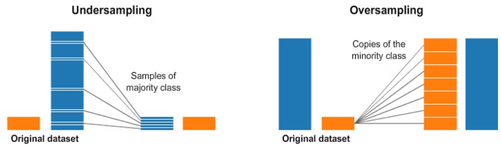
\includegraphics[width=0.8\linewidth]{16.png}
    %\fbox{\parbox[c][4cm][c]{0.8\linewidth}{\centering \textit{[Chèn ảnh: Minh họa Over-sampling (SMOTE / ADASYN) tại đây]}}}
    \caption{Các kỹ thuật cân bằng dữ liệu}
    \label{fig:balance_data}
\end{figure}

\begin{itemize}
    \item Mục đích: Làm cho dữ liệu đỡ bị mất cân bằng giữa các lớp.
    \item \textbf{Over-sampling:} Tăng mức độ tiếp xúc với phần dữ liệu thiểu số:
    \begin{itemize}
        \item \textbf{Nhân bản hóa (RandomOverSampler):} Nhân bản các thành phần thiểu số $\rightarrow$ số lượng tăng lên nhưng độ đa dạng không đổi.
        \item \textbf{Tổng hợp (SMOTE và ADASYN):}
        \begin{itemize}
            \item \textbf{SMOTE} (\textit{Synthetic Minority Oversampling Technique}): Hoạt động bằng cách chọn các điểm thuộc nhóm thiểu số gần điểm ban đầu, nội suy ra đường thẳng nối từ điểm $A$ đến điểm $B$ và chọn ngẫu nhiên một điểm nằm trên đường thẳng đó (trọng số của điểm mới dựa trên sự nội suy giữa $A$ và $B$).
            \item \textbf{ADASYN} (\textit{Adaptive Synthetic Sampling}): Hoạt động dựa trên việc sinh ra điểm nhân tạo từ các \textbf{điểm khó học} (điểm khó học là điểm bị bao quanh bởi nhiều điểm thuộc nhóm đa số $\rightarrow$ tính trọng số dựa trên các điểm đa số xung quanh, trọng số càng cao thì càng khó học; sau đó tiếp tục dùng kỹ thuật tương tự SMOTE để sinh ra điểm thiểu số nhân tạo).
        \end{itemize}
    \end{itemize}
    \item \textbf{Under-sampling:} Làm giảm phần dữ liệu đa số.
    \item $\rightarrow$ \textbf{Kết luận:} Chuộng \textbf{Over-sampling} hơn thay vì Under-sampling vì dữ liệu luôn cần được bảo toàn thay vì làm mất đi như Under-sampling.
\end{itemize}

% ==========================================
% SECTION 5: TRỰC QUAN HÓA DỮ LIỆU TRONG PYTHON
% ==========================================
\section{Data Visualization trong Python}

\begin{figure}[H]
    \centering
    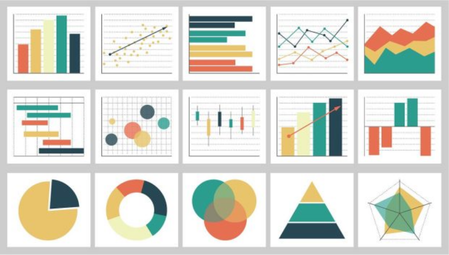
\includegraphics[width=0.8\linewidth]{17.png}
    %\fbox{\parbox[c][4cm][c]{0.8\linewidth}{\centering \textit{[Chèn ảnh: Các loại biểu đồ trực quan hóa dữ liệu tại đây]}}}
    \caption{Phân loại các biểu đồ trực quan hóa dữ liệu}
    \label{fig:data_vis}
\end{figure}

\begin{itemize}
    \item \textbf{Các thư viện phổ biến:} \texttt{numpy}, \texttt{matplotlib}, \texttt{pandas}, \texttt{seaborn}.
    \item \textbf{Các loại biểu đồ thường dùng:}
    \begin{itemize}
        \item Histogram
        \item Density plot (biểu diễn phân phối liên tục)
        \item Box plot
        \item Correlation matrix plot
        \item Scatter matrix plot
    \end{itemize}
    \item \textbf{Một số thành phần trong Matplotlib:}
    \begin{itemize}
        \item \texttt{grid}: Dóng cột và hàng (lưới tọa độ).
        \item \texttt{legend}: Chú thích (hữu ích khi một đồ thị có nhiều đường).
    \end{itemize}
\end{itemize}  <-- Tuần sau học thì bỏ dấu % đi

\end{document}